\documentclass[tikz,border=14pt]{standalone}
\usepackage{amsmath,amssymb}
\usetikzlibrary{arrows.meta,decorations.markings,calc,backgrounds,matrix}

\begin{document}
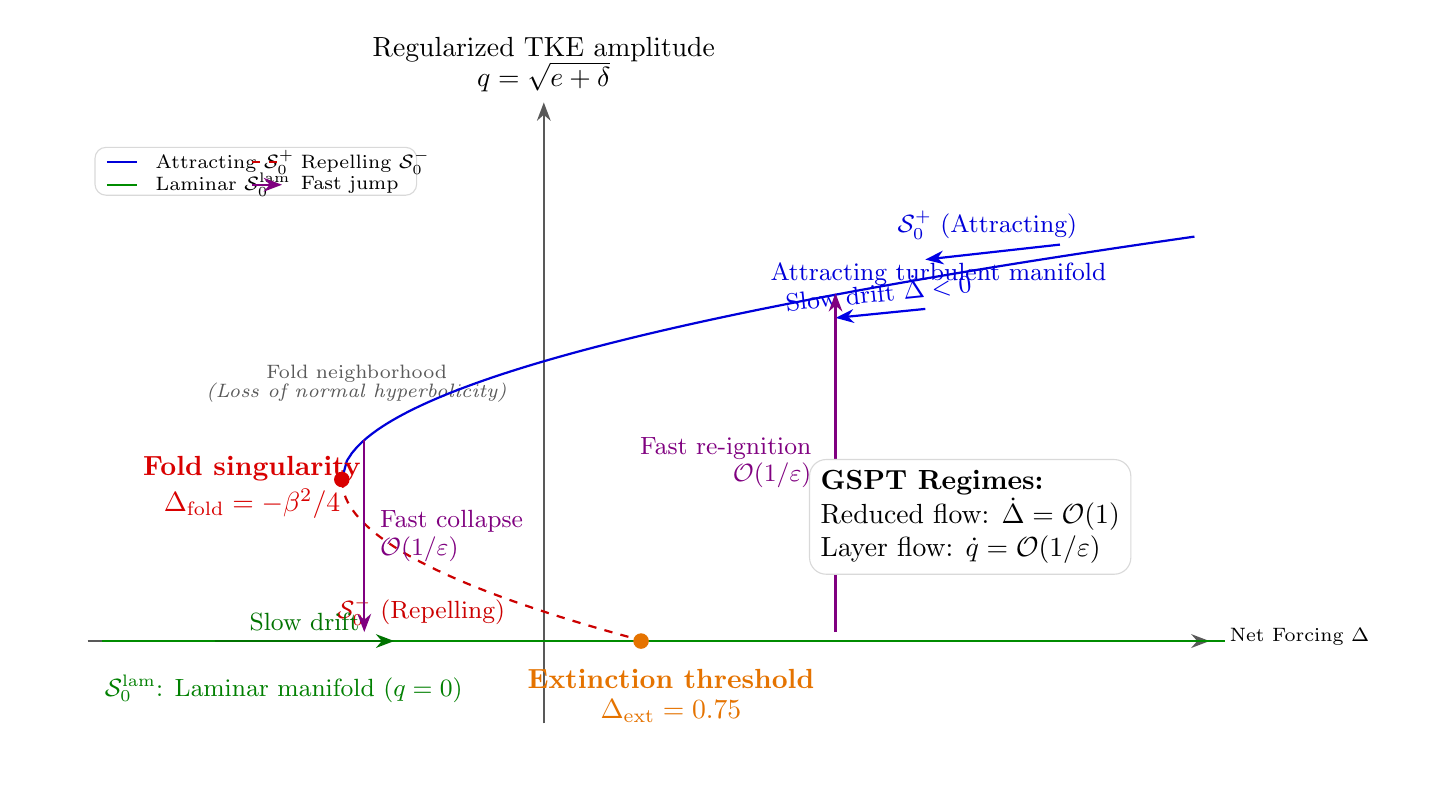
\begin{tikzpicture}[x=1.9cm,y=1.9cm,>=Stealth,font=\scriptsize]

    % --- Key coordinates ---
    \coordinate (Fold) at (-1.35, 1.08);
    \coordinate (Extinction) at (0.65, 0.00);

    % --- White canvas to avoid transparent/black preview backgrounds ---
    \fill[white] (-3.45,-0.85) rectangle (5.75,4.10);

    % --- Axes ---
    \draw[->, thick, gray!70!black] (-3.05,0.00) -- (4.45,0.00);
    \node[anchor=west, black] at (4.52,0.03) {Net Forcing $\Delta$};
    \draw[->, thick, gray!70!black] (0.00,-0.55) -- (0.00,3.60)
        node[above, align=center, black, font=\normalsize] {Regularized TKE amplitude\\[-1pt]$q=\sqrt{e+\delta}$};

    % --- Fold neighborhood ---
    \begin{scope}[on background layer]
        \filldraw[fill=gray!14, draw=gray!50, dashed] (Fold) circle (0.42);
    \end{scope}
    \node[gray!70!black, font=\scriptsize, align=center] at (-1.25,1.72)
        {Fold neighborhood\\[-1pt]\textit{(Loss of normal hyperbolicity)}};

    % --- Legend (manual 2x2 layout for reliable text rendering) ---
    \draw[rounded corners=4pt, draw=gray!30, fill=white] (-3.00,2.98) rectangle (-0.85,3.30);
    \draw[thick, blue!85!black] (-2.92,3.20) -- (-2.72,3.20);
    \node[anchor=west] at (-2.66,3.20) {Attracting $\mathcal{S}_0^+$};
    \draw[thick, dashed, red!80!black] (-1.95,3.20) -- (-1.75,3.20);
    \node[anchor=west] at (-1.69,3.20) {Repelling $\mathcal{S}_0^-$};
    \draw[thick, green!55!black] (-2.92,3.05) -- (-2.72,3.05);
    \node[anchor=west] at (-2.66,3.05) {Laminar $\mathcal{S}_0^{\mathrm{lam}}$};
    \draw[->, thick, violet] (-1.95,3.05) -- (-1.75,3.05);
    \node[anchor=west] at (-1.69,3.05) {Fast jump};

    % --- Manifolds ---
    \draw[thick, green!55!black] (-2.95,0.00) -- (4.55,0.00);
    \node[green!50!black, anchor=north west, font=\small] at (-3.00,-0.16)
        {$\mathcal{S}_0^{\mathrm{lam}}$: Laminar manifold ($q=0$)};

    \draw[thick, dashed, red!80!black, domain=-1.35:0.65, samples=150]
        plot ({\x}, {1.08 - 0.76*sqrt(\x + 1.35)});
    \node[red!80!black, font=\small] at (-0.82,0.20)
        {$\mathcal{S}_0^-$ (Repelling)};

    \draw[thick, blue!85!black, domain=-1.35:4.35, samples=170]
        plot ({\x}, {1.08 + 0.68*sqrt(\x + 1.35)});
    \node[blue!85!black, font=\small, anchor=west] at (2.30,2.78)
        {$\mathcal{S}_0^+$ (Attracting)};
    \node[blue!85!black, font=\small, anchor=west] at (1.45,2.45)
        {Attracting turbulent manifold};

    % --- Slow drift arrows ---
    \draw[->, thick, blue!90!black] (3.45,2.65) -- (2.55,2.55);
    \draw[->, thick, blue!90!black] (2.55,2.22) -- (1.95,2.16)
        node[midway, above, sloped, font=\small] {Slow drift $\dot{\Delta}<0$};
    \draw[->, thick, green!45!black] (-2.20,0.00) -- (-1.00,0.00)
        node[midway, above, font=\small] {Slow drift};

    % --- Fast jumps ---
    \pgfmathsetmacro{\qcollapse}{1.08 + 0.68*sqrt(-1.20 + 1.35)}
    \draw[->, thick, violet] (-1.20,\qcollapse) -- (-1.20,0.06)
        node[midway, right=2pt, align=left, font=\small] {Fast collapse\\[-1pt]$\mathcal{O}(1/\varepsilon)$};

    \pgfmathsetmacro{\qreignite}{1.08 + 0.68*sqrt(2.0 + 1.35)}
    \draw[->, thick, violet] (1.95,0.06) -- (1.95,\qreignite)
        node[midway, left=5pt, align=right, font=\small] {Fast re-ignition\\[-1pt]$\mathcal{O}(1/\varepsilon)$};

    % --- Threshold points and labels ---
    \filldraw[red!85!black] (Fold) circle (2.6pt);
    \node[red!85!black, font=\normalsize, align=right] at (-1.95,1.15)
        {\textbf{Fold singularity}};
    \node[red!85!black, font=\normalsize, align=right] at (-1.95,0.92)
        {$\Delta_{\mathrm{fold}}=-\beta^2/4$};

    \filldraw[orange!90!black] (Extinction) circle (2.6pt);
    \node[orange!90!black, font=\normalsize, align=left] at (0.85,-0.25)
        {\textbf{Extinction threshold}};
    \node[orange!90!black, font=\normalsize, align=left] at (0.85,-0.47)
        {$\Delta_{\mathrm{ext}}=0.75$};

    % --- Regime box ---
    \node[
        draw=gray!30,
        fill=white,
        rounded corners=6pt,
        inner sep=4pt,
        align=left,
        font=\normalsize
    ] at (2.85,0.83) {
        \textbf{GSPT Regimes:}\\
        Reduced flow: $\dot{\Delta}=\mathcal{O}(1)$\\
        Layer flow: $\dot{q}=\mathcal{O}(1/\varepsilon)$
    };

\end{tikzpicture}
\end{document}